\documentclass[12pt]{article}
\usepackage[margin=0.75in]{geometry}
\usepackage{float}
\usepackage{multicol}
\usepackage{lmodern}
\usepackage{amssymb,amsmath}
\usepackage{ifxetex,ifluatex}
\usepackage{fixltx2e} % provides \textsubscript
\ifnum 0\ifxetex 1\fi\ifluatex 1\fi=0 % if pdftex
  \usepackage[T1]{fontenc}
  \usepackage[utf8]{inputenc}
\else % if luatex or xelatex
  \ifxetex
    \usepackage{mathspec}
    \usepackage{xltxtra,xunicode}
  \else
    \usepackage{fontspec}
  \fi
  \defaultfontfeatures{Mapping=tex-text,Scale=MatchLowercase}
  \newcommand{\euro}{€}
\fi
% use upquote if available, for straight quotes in verbatim environments
\IfFileExists{upquote.sty}{\usepackage{upquote}}{}
% use microtype if available
\IfFileExists{microtype.sty}{%
\usepackage{microtype}
\UseMicrotypeSet[protrusion]{basicmath} % disable protrusion for tt fonts
}{}
\usepackage{graphicx}
\makeatletter
\def\maxwidth{\ifdim\Gin@nat@width>\linewidth\linewidth\else\Gin@nat@width\fi}
\def\maxheight{\ifdim\Gin@nat@height>\textheight\textheight\else\Gin@nat@height\fi}
\makeatother
% Scale images if necessary, so that they will not overflow the page
% margins by default, and it is still possible to overwrite the defaults
% using explicit options in \includegraphics[width=3.5in][width, height, ...]{}
\setkeys{Gin}{width=\maxwidth,height=\maxheight,keepaspectratio}
\ifxetex
  \usepackage[setpagesize=false, % page size defined by xetex
              unicode=false, % unicode breaks when used with xetex
              xetex]{hyperref}
\else
  \usepackage[unicode=true]{hyperref}
\fi
\hypersetup{breaklinks=true,
            bookmarks=true,
            pdfauthor={Brandon LeBeau},
            pdftitle={PSQF 4143: Section 13},
            colorlinks=true,
            citecolor=blue,
            urlcolor=blue,
            linkcolor=magenta,
            pdfborder={0 0 0}}
\urlstyle{same}  % don't use monospace font for urls
\setlength{\parindent}{0pt}
\setlength{\parskip}{6pt plus 2pt minus 1pt}
\setlength{\emergencystretch}{3em}  % prevent overfull lines
\setcounter{secnumdepth}{0}

\title{PSQF 4143: Section 13}
\author{Brandon LeBeau}
\date{}

\begin{document}
\maketitle

\section{Correlation Introduction}\label{correlation-introduction}

\begin{itemize}
\itemsep1pt\parskip0pt\parsep0pt
\item
  Up to now, we have primarily focused on statistics for single
  variables
\item
  We will now shift to discuss how to quantify and explore the
  relationship between two variables.
\item
  To display the relationship between two variables, could use a
  bivariate frequency distribution or a scatterplot.
\end{itemize}

\section{Bivariate Frequency
Distribution}\label{bivariate-frequency-distribution}

\begin{figure}[H]
\centering
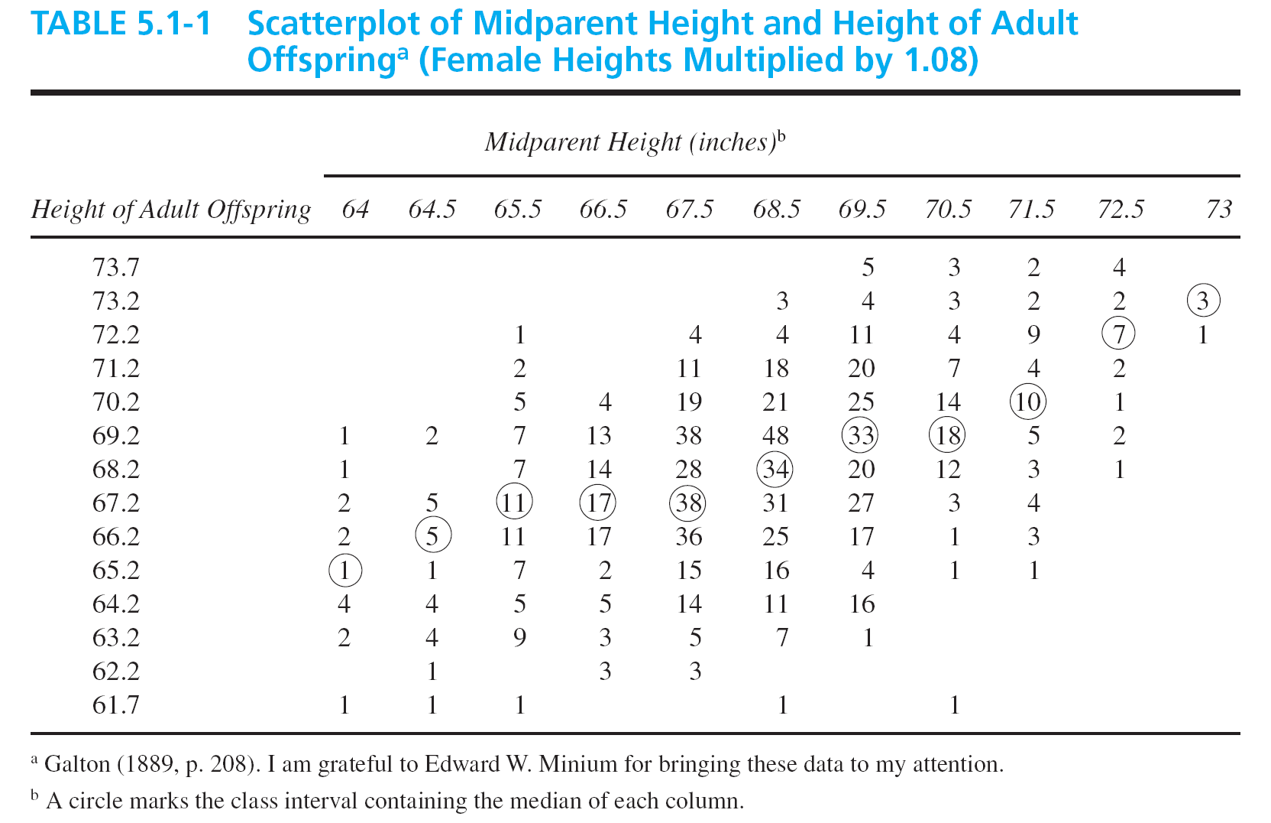
\includegraphics[width=3.5in]{bivariate_freq.png}
\caption{}
\end{figure}

\section{Scatterplot}\label{scatterplot}

\begin{figure}[H]
\centering
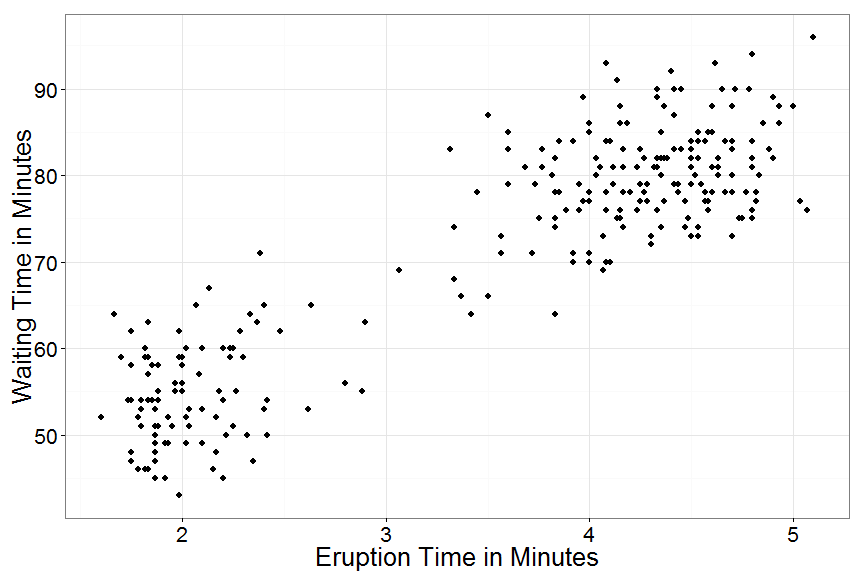
\includegraphics[width=3.5in]{figure/eruptions-1.png}
\caption{plot of chunk eruptions}
\end{figure}

\begin{figure}[H]
\centering
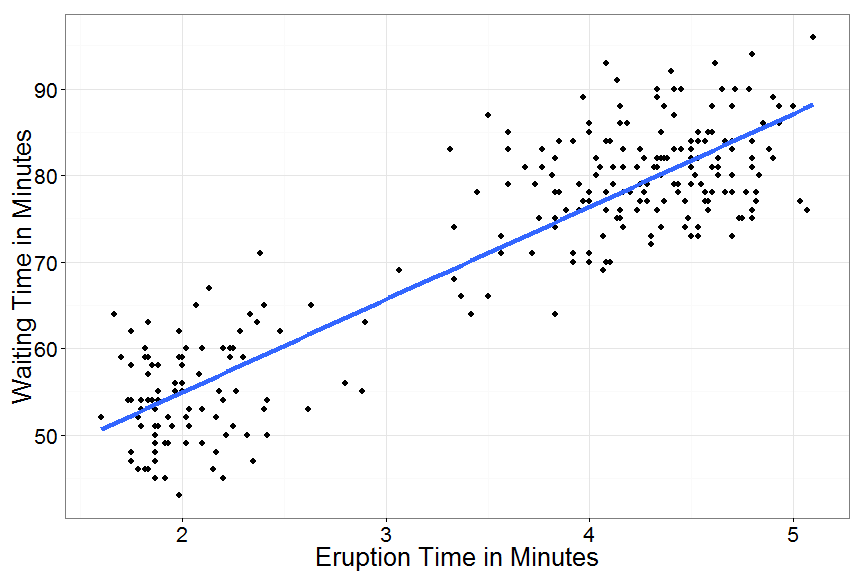
\includegraphics[width=3.5in]{figure/eruptionslinear-1.png}
\caption{plot of chunk eruptionslinear}
\end{figure}

\section{Correlation 2}\label{correlation-2}

\begin{itemize}
\itemsep1pt\parskip0pt\parsep0pt
\item
  The correlation gives us a measure to describe the relationship
  between two variables.

  \begin{itemize}
  \itemsep1pt\parskip0pt\parsep0pt
  \item
    The form of the relationship
  \item
    The direction of the relationship
  \item
    The strength of the relationship
  \end{itemize}
\item
  The pearson product-moment correlation coefficient (correlation)
  describes the amount of \textbf{linear} relationship between two
  variables.
\item
  Notation:

  \begin{itemize}
  \itemsep1pt\parskip0pt\parsep0pt
  \item
    Sample: \(r\)
  \item
    Population: \(\rho\)
  \end{itemize}
\end{itemize}

\section{Correlation 3}\label{correlation-3}

\begin{itemize}
\itemsep1pt\parskip0pt\parsep0pt
\item
  Correlations can be either positive or negative:

  \begin{itemize}
  \itemsep1pt\parskip0pt\parsep0pt
  \item
    Positive: Effort and Achievement -- People who expend more effort
    tend to achieve more.
  \item
    Negative: Cholesterol level and life expectancy -- People with lower
    cholesterol levels tend to live longer.
  \end{itemize}
\item
  A correlation of 1 represents a perfect positive relationship.

  \begin{itemize}
  \itemsep1pt\parskip0pt\parsep0pt
  \item
    Example: Annual precipitation in inches and annual precipitation in
    centimeters.
  \end{itemize}
\item
  A correlation of -1 represents a perfect negative relationship.

  \begin{itemize}
  \itemsep1pt\parskip0pt\parsep0pt
  \item
    Example: Number of days in class and number of days absent.
  \end{itemize}
\item
  A correlation of 0 represents no relationship.

  \begin{itemize}
  \itemsep1pt\parskip0pt\parsep0pt
  \item
    Example: height and last digit of social security number.
  \end{itemize}
\end{itemize}

\section{Examples}\label{examples}

\begin{figure}[H]
\centering
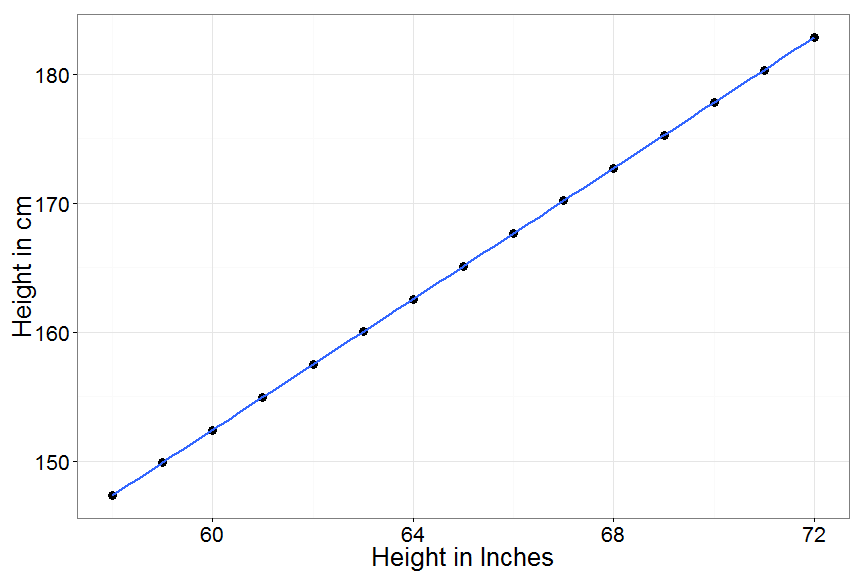
\includegraphics[width=3.5in]{figure/height-1.png}
\caption{plot of chunk height}
\end{figure}

\begin{figure}[H]
\centering
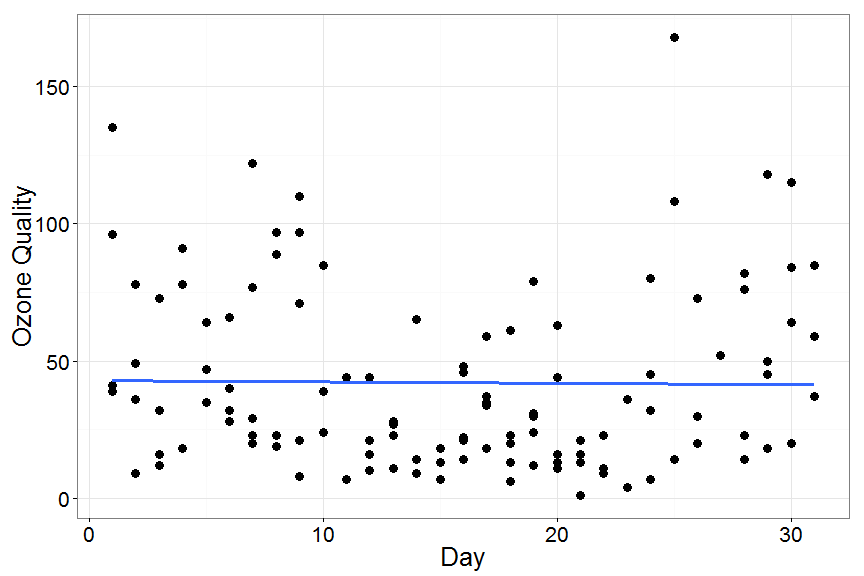
\includegraphics[width=3.5in]{figure/ozone-1.png}
\caption{plot of chunk ozone}
\end{figure}

\section{Real world Examples}\label{real-world-examples}

\begin{figure}[H]
\centering
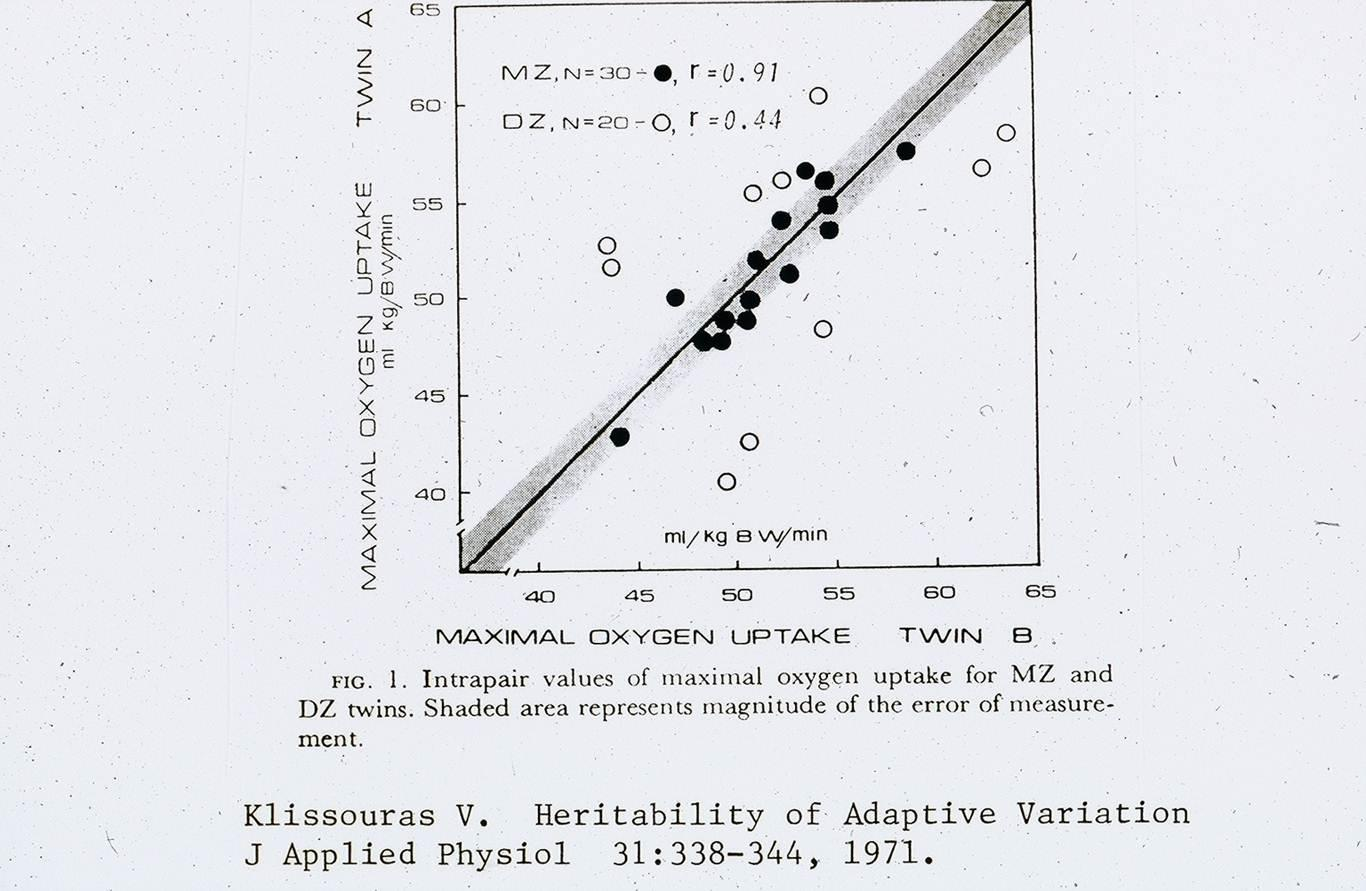
\includegraphics[width=3.5in]{twins.jpg}
\caption{Twins}
\end{figure}

\section{Real World Example 2}\label{real-world-example-2}

\begin{figure}[H]
\centering
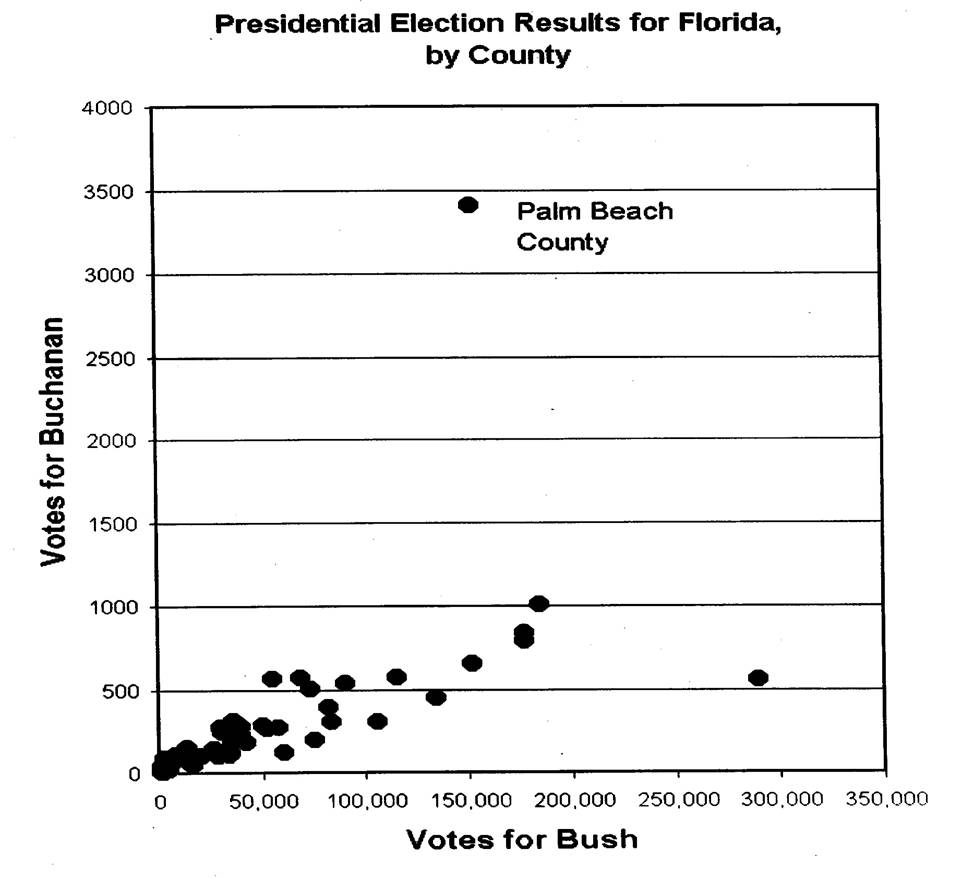
\includegraphics[width=3.5in]{floridaBB.jpg}
\caption{Florida Election}
\end{figure}

\section{Real World Example 2 cont.}\label{real-world-example-2-cont.}

\begin{figure}[H]
\centering
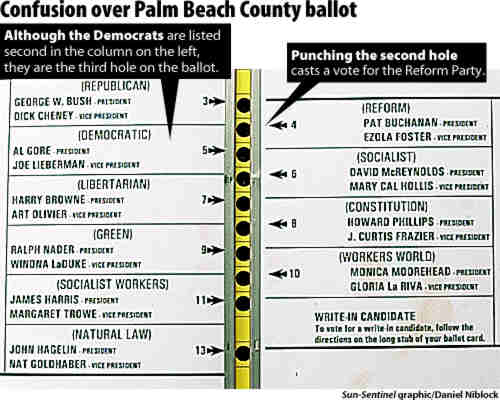
\includegraphics[width=3.5in]{palmballot.jpg}
\caption{ballot}
\end{figure}

\section{Guessing Correlations}\label{guessing-correlations}

http://istics.net/stat/Correlations/

\section{Correlation Formula}\label{correlation-formula}

\[ r = \frac{\mbox{degree to which X and Y vary together}}{\mbox{degree to which X and Y vary separately}} \]

\[ r = \frac{s_{XY}}{s_{X}s_{Y}} = \frac{\sum(X-\bar{X})(Y-\bar{Y})}{s_{X}s_{Y}}*\frac{1}{n} \]

where \(s_{XY} = \frac{\sum(X-\bar{X})(Y-\bar{Y})}{n}\) is the
\textbf{covariance}\\and \(s_{X}\) and \(s_{Y}\) are the standard
deviations of the \(X\) and \(Y\) respectively.

\[ r = \frac{\sum z_{x} z_{y}}{n} \]

\section{Calculating the Correlation}\label{calculating-the-correlation}

\begin{figure}[H]
\centering
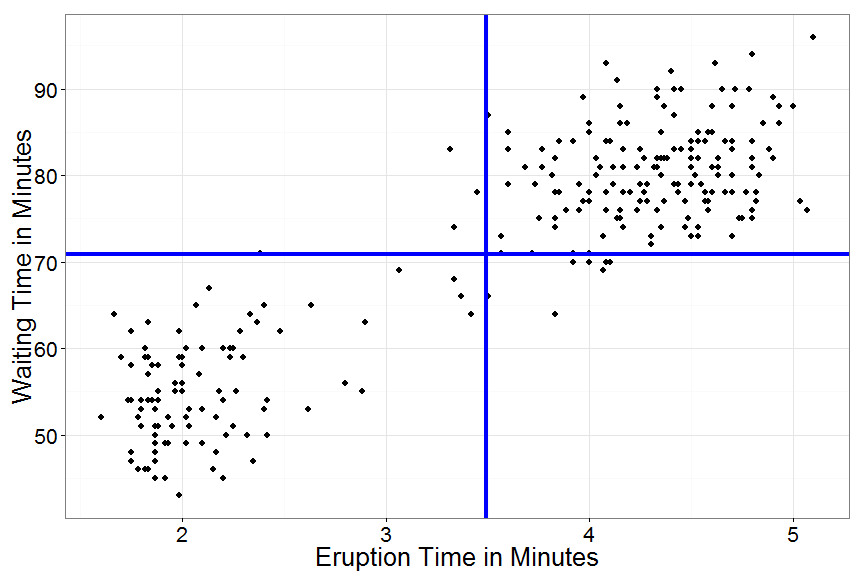
\includegraphics[width=3.5in]{figure/faithful2-1.png}
\caption{plot of chunk faithful2}
\end{figure}

\section{Correlation Formula 2}\label{correlation-formula-2}

\begin{itemize}
\itemsep1pt\parskip0pt\parsep0pt
\item
  Formula for raw scores:
  \[ r = \frac{\sum (X - \bar{X})(Y- \bar{Y})}{(n)s_{x}s_{y}} \]
  \[ \rho = \frac{\sum (X - \mu_{X})(Y- \mu_{Y})}{(N)\sigma_{x}\sigma_{y}} \]
\end{itemize}

\section{Correlation Properties}\label{correlation-properties}

\begin{enumerate}
\def\labelenumi{\arabic{enumi}.}
\itemsep1pt\parskip0pt\parsep0pt
\item
  \(r\) ranges from -1 (perfect negative relationship) to +1 (perfect
  positive relationship)
\item
  \(r = 0\) when there is no \textbf{linear} relationship between the
  variables.
\item
  The closer \(r\) is to +1 or -1, the stronger the relationship

  \begin{itemize}
  \itemsep1pt\parskip0pt\parsep0pt
  \item
    For example, \(r = -0.7\) is stronger than \(r = 0.49\).
  \end{itemize}
\item
  Changes in the scale are not uniform.

  \begin{itemize}
  \itemsep1pt\parskip0pt\parsep0pt
  \item
    For example, a change from \(r = 0.4\) does not represent half the
    relationship as \(r = 0.8\)
  \end{itemize}
\end{enumerate}

\section{Correlation Properties 2}\label{correlation-properties-2}

\begin{enumerate}
\def\labelenumi{\arabic{enumi}.}
\setcounter{enumi}{4}
\itemsep1pt\parskip0pt\parsep0pt
\item
  Linear transformations do not impact the correlation.

  \begin{itemize}
  \itemsep1pt\parskip0pt\parsep0pt
  \item
    Example, the corelation between the temperatures in Boston and New
    York would be identical on Fahrenheit or Celsius scales
  \end{itemize}
\end{enumerate}

\begin{figure}[H]
\centering
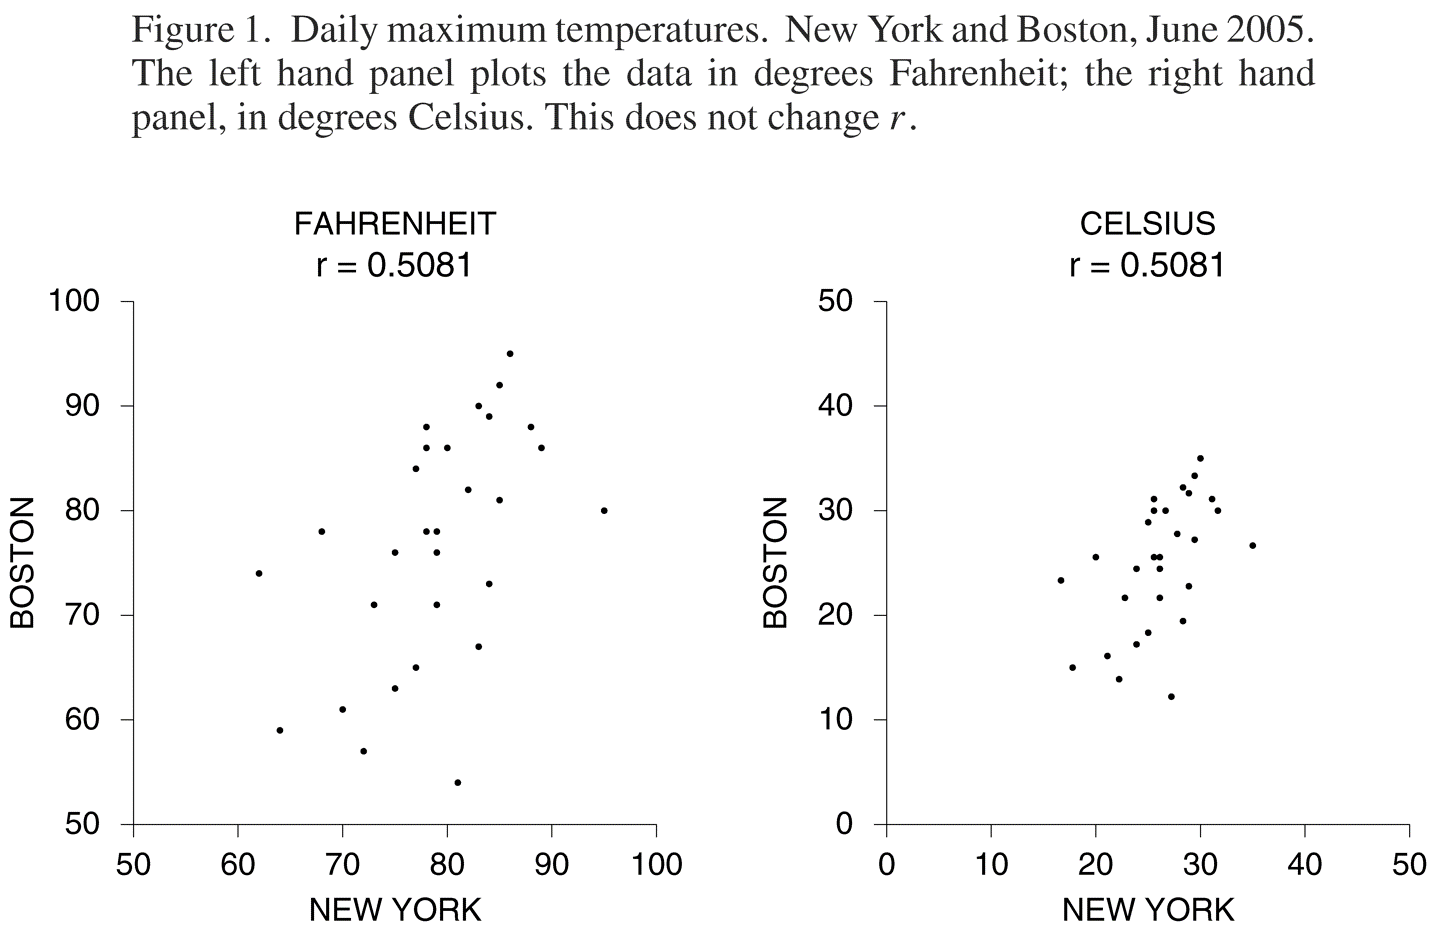
\includegraphics[width=3.5in]{linear_corr.png}
\caption{}
\end{figure}

\begin{enumerate}
\def\labelenumi{\arabic{enumi}.}
\setcounter{enumi}{5}
\itemsep1pt\parskip0pt\parsep0pt
\item
  Flipping the X and Y variables does not change the correlation.
\end{enumerate}

\begin{figure}[H]
\centering
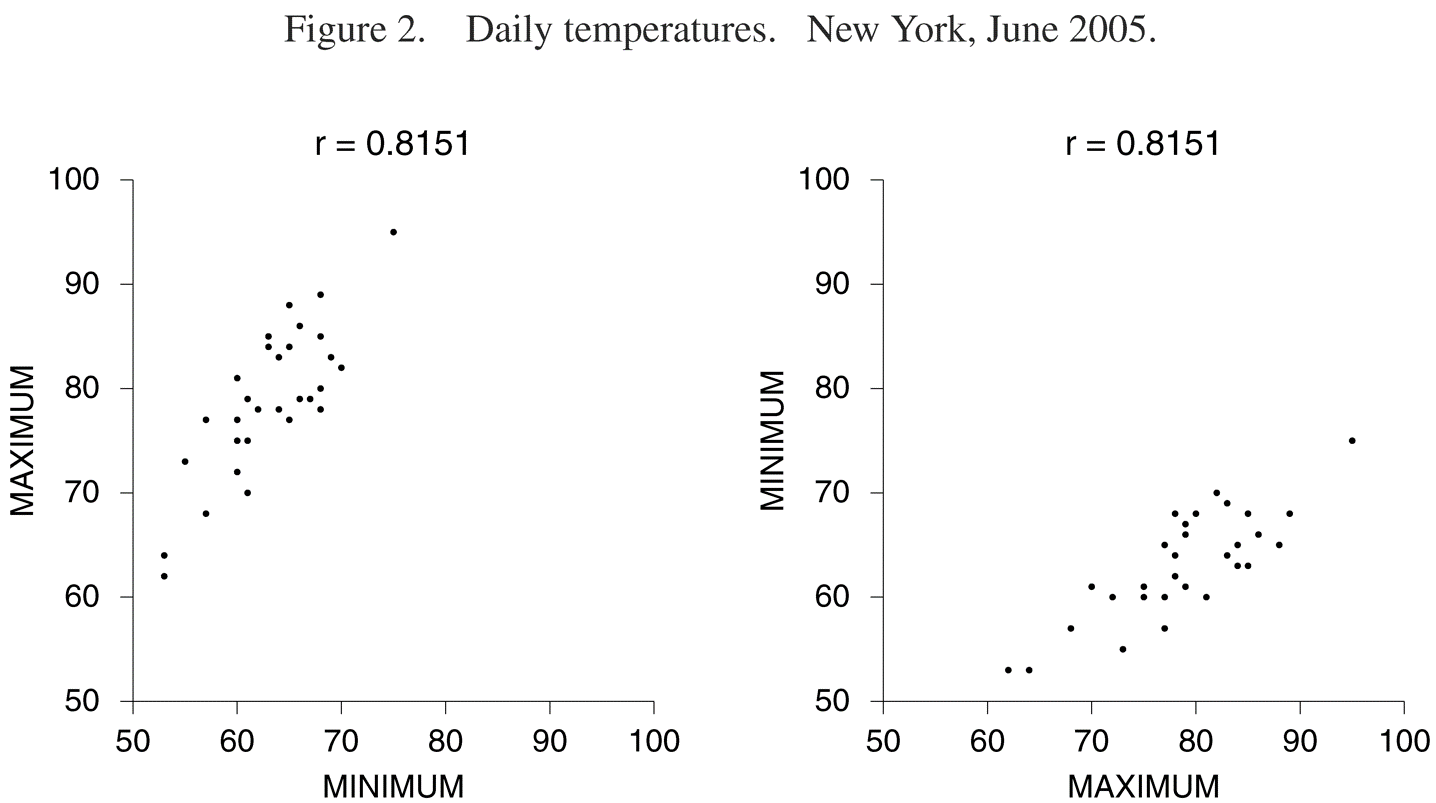
\includegraphics[width=3.5in]{flip_xy_corr.png}
\caption{}
\end{figure}

\section{Perfect Linearity}\label{perfect-linearity}

\begin{itemize}
\itemsep1pt\parskip0pt\parsep0pt
\item
  Perfect linearity does not always imply perfect correlation.
\end{itemize}

\begin{figure}[H]
\centering
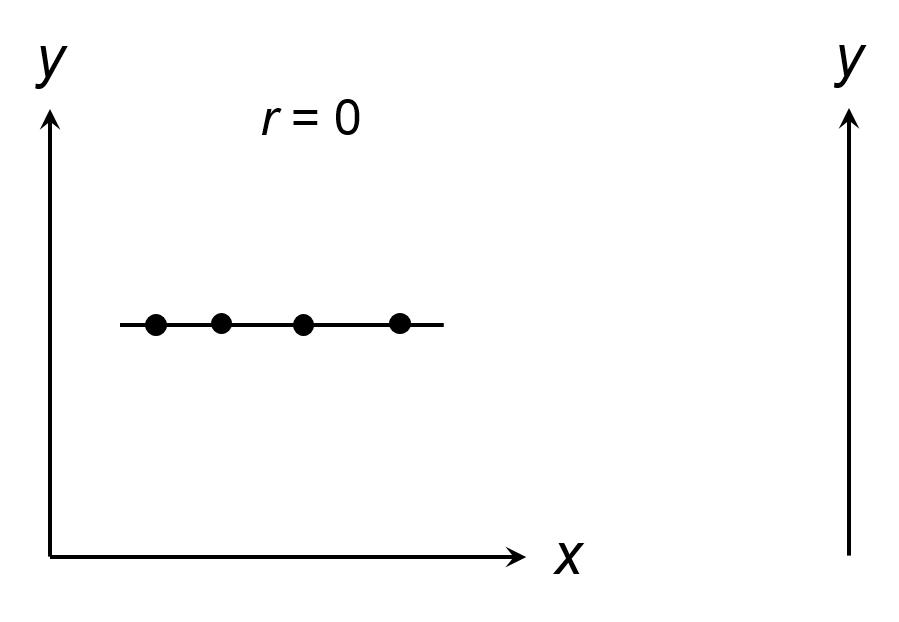
\includegraphics[width=3.5in]{perfect_nocorr.png}
\caption{}
\end{figure}

\section{Non-linear Trends}\label{non-linear-trends}

\begin{itemize}
\itemsep1pt\parskip0pt\parsep0pt
\item
  Remember that the correlation we have discussed measures the
  \textbf{linear} relationship, not non-linear.
\end{itemize}

\begin{figure}[H]
\centering
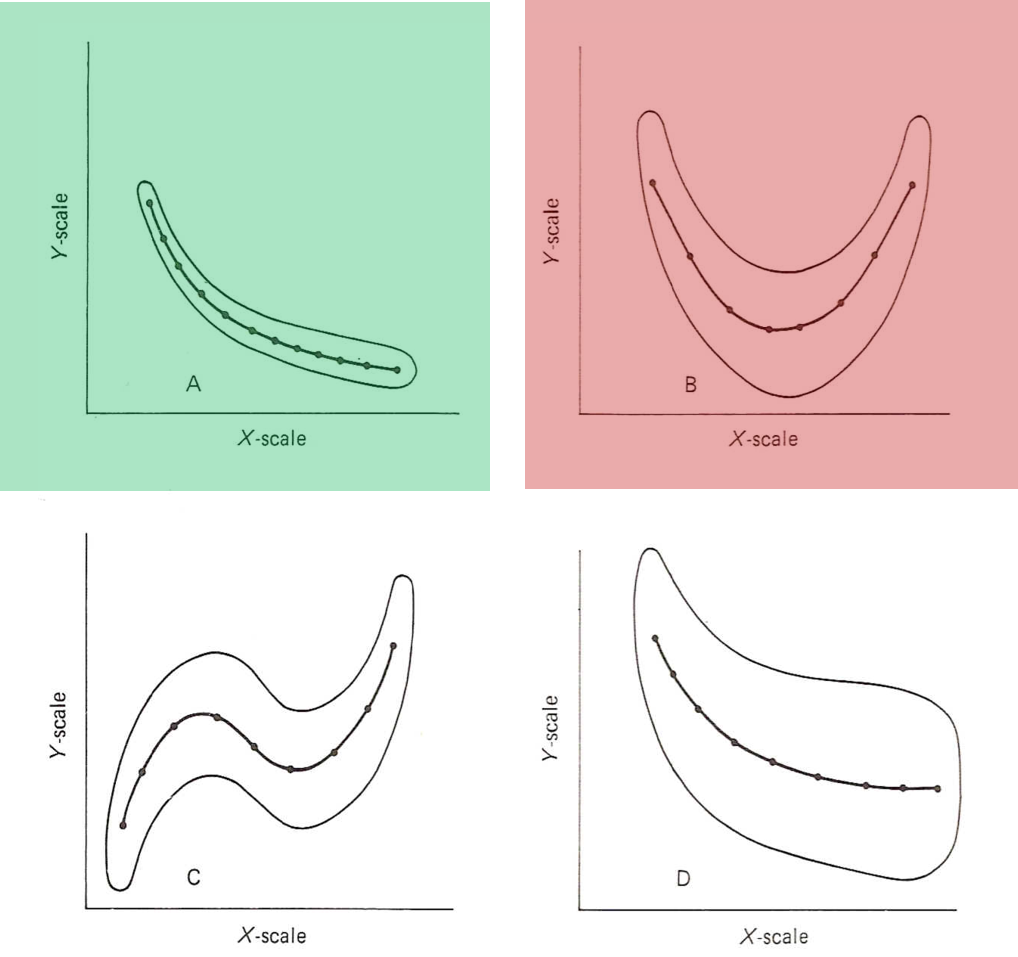
\includegraphics[width=3.5in]{nonlinear.png}
\caption{}
\end{figure}

\section{Interpretation of the
Correlation}\label{interpretation-of-the-correlation}

\begin{itemize}
\itemsep1pt\parskip0pt\parsep0pt
\item
  Assuming linearity exists, what does \(r = 0.75\) mean?
\end{itemize}

\begin{enumerate}
\def\labelenumi{\arabic{enumi}.}
\itemsep1pt\parskip0pt\parsep0pt
\item
  Interpret \(r\) in an absolute sense (can be troublesome out of
  context):

  \begin{itemize}
  \itemsep1pt\parskip0pt\parsep0pt
  \item
    \(| r | > 0.75\); strong correlation
  \item
    \(| r | > 0.3\); medium correlation
  \item
    \(| r | < 0.3\); weak correlation
  \end{itemize}
\item
  Interpret in a relative sense:

  \begin{itemize}
  \itemsep1pt\parskip0pt\parsep0pt
  \item
    Parallel test forms (Form A -- Form B); \(r = 0.75\) is low
  \item
    ACT to Freshman GPA; \(r = 0.75\) is high
  \end{itemize}
\end{enumerate}

\section{Interpretation of the Correlation
2}\label{interpretation-of-the-correlation-2}

\begin{enumerate}
\def\labelenumi{\arabic{enumi}.}
\setcounter{enumi}{2}
\itemsep1pt\parskip0pt\parsep0pt
\item
  \(r^2\) is an indication of the amount of variability one variable
  explains in the other variable.

  \begin{itemize}
  \itemsep1pt\parskip0pt\parsep0pt
  \item
    Example: \(r = 0.75\), \(r^2 = 0.56\); 56\% of the variation in Y is
    explained by X.
  \end{itemize}
\item
  \(r\) as an index of prediction accuracy.
\end{enumerate}

\begin{figure}[H]
\centering
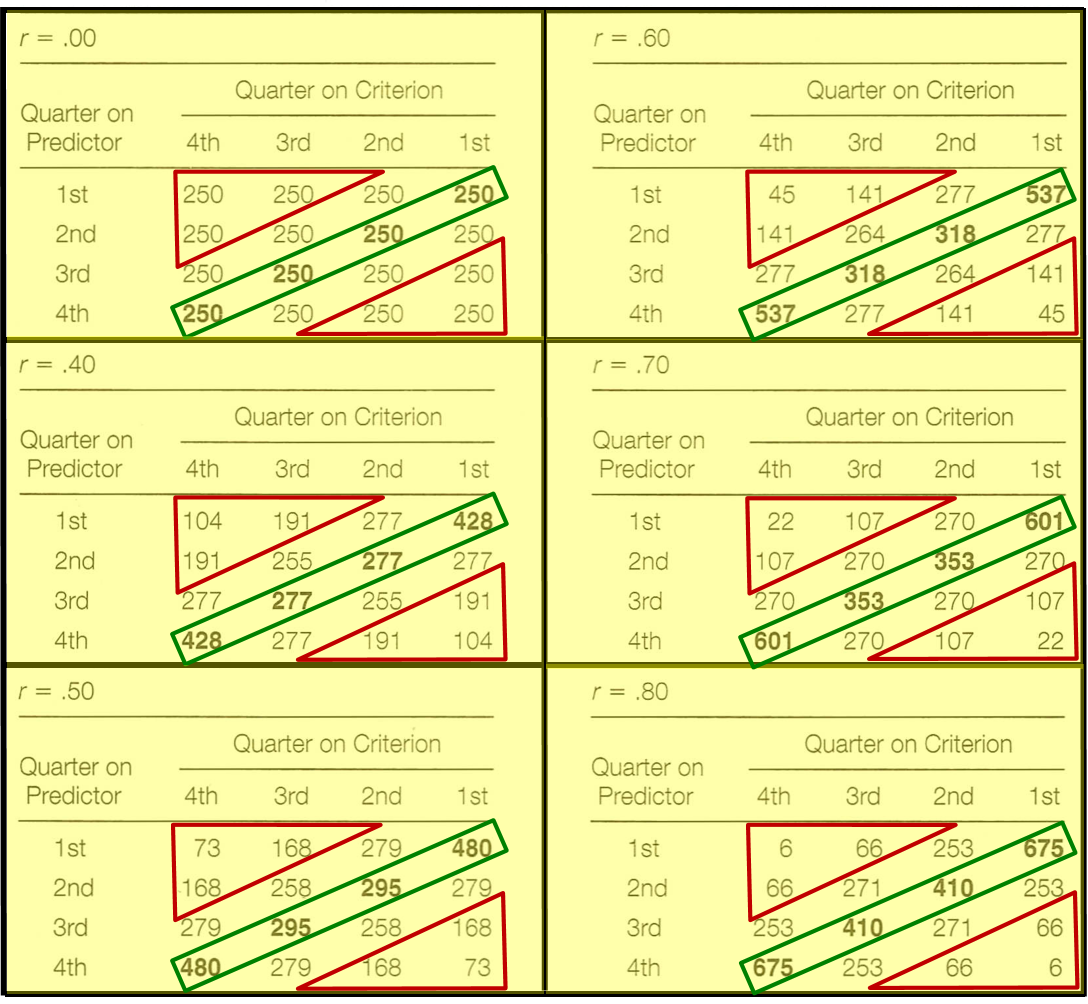
\includegraphics[width=3.5in]{corr_predaccur.png}
\caption{}
\end{figure}

\section{Correlation is not
Causation}\label{correlation-is-not-causation}

\begin{itemize}
\itemsep1pt\parskip0pt\parsep0pt
\item
  We find a relationship between X and Y

  \begin{itemize}
  \itemsep1pt\parskip0pt\parsep0pt
  \item
    This relationship may be that X \textbf{causes} Y
  \item
    Or it could be that Y \textbf{causes} X
  \item
    It could be that a third variable causes both X and Y
  \end{itemize}
\item
  Most likely, there is a complex web of variables that are at play.
\end{itemize}

\section{Confounding}\label{confounding}

\begin{itemize}
\itemsep1pt\parskip0pt\parsep0pt
\item
  Confounding is when Y is caused by X and a third variable (but the
  third variable is not related to X). Therefore, the effect of X is
  confounded with a third variables
\end{itemize}

\begin{figure}[H]
\centering
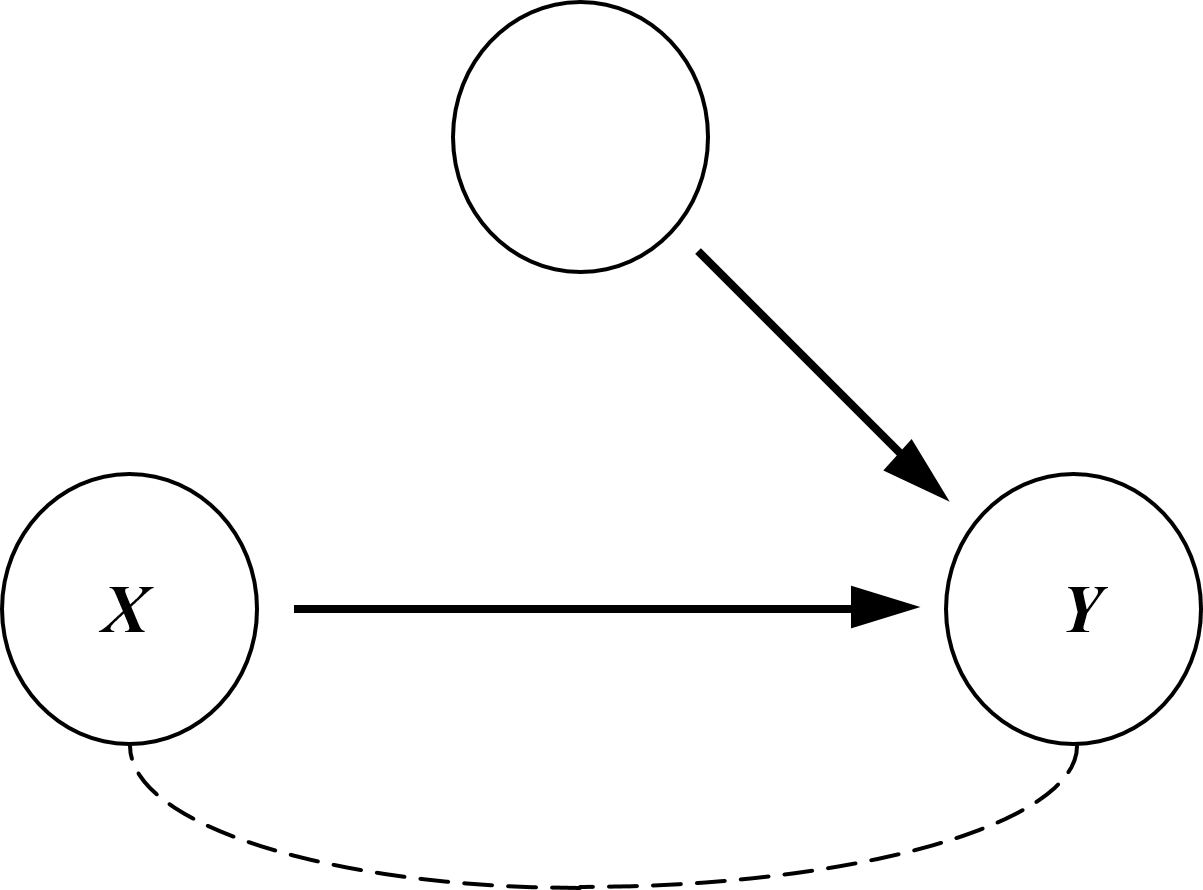
\includegraphics[width=3.5in]{confounding.png}
\caption{}
\end{figure}

\section{Correlation with time}\label{correlation-with-time}

\begin{figure}[H]
\centering
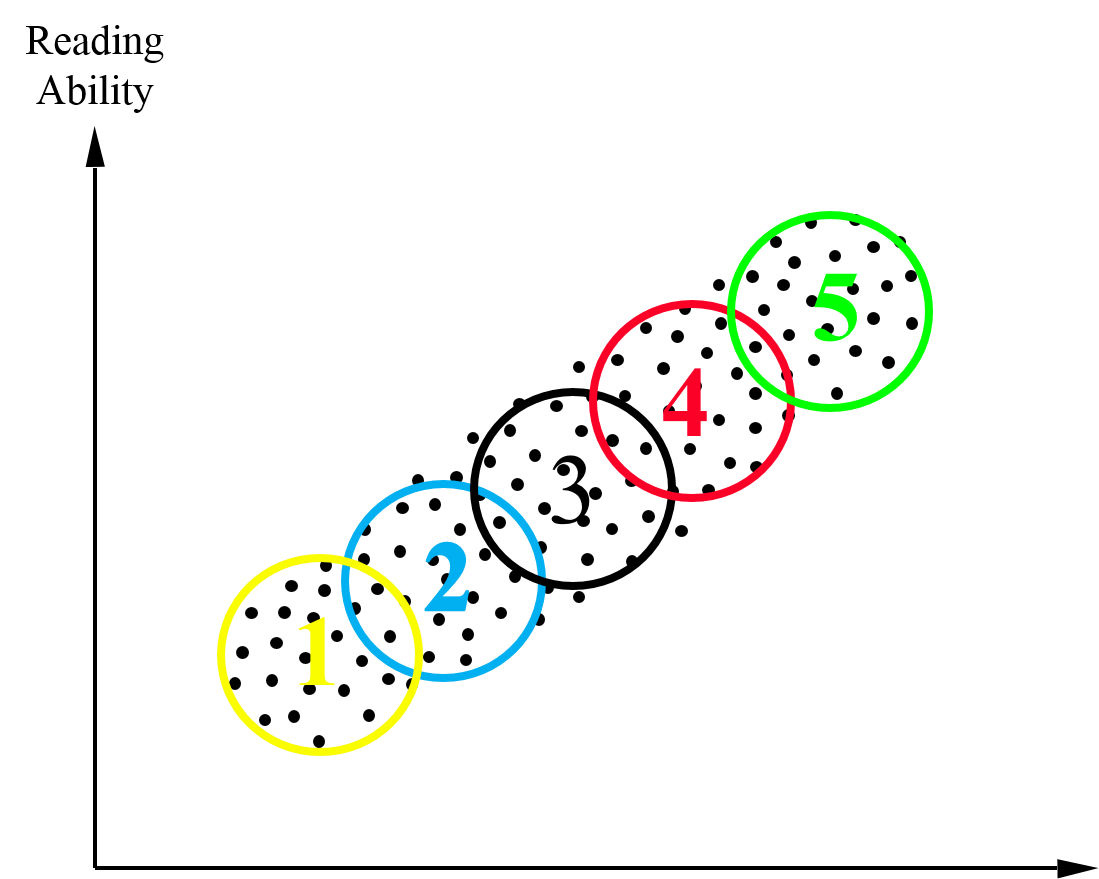
\includegraphics[width=3.5in]{corr_time.png}
\caption{}
\end{figure}

\section{Correlation is not Causation
Summary}\label{correlation-is-not-causation-summary}

\begin{itemize}
\itemsep1pt\parskip0pt\parsep0pt
\item
  Correlation specifically measures association/relationships
\item
  Being associated or related is not the same as causation
\item
  Inferences about causation can only be made with logic and careful
  experimental design/control.
\item
  The value of \(r\) itself can not be used for causation
\end{itemize}

\section{Restriction of Range}\label{restriction-of-range}

\begin{itemize}
\itemsep1pt\parskip0pt\parsep0pt
\item
  Restriction of range can have the effect of decreasing the
  correlation.
\item
  This happens due to decreasing the variability.
\end{itemize}

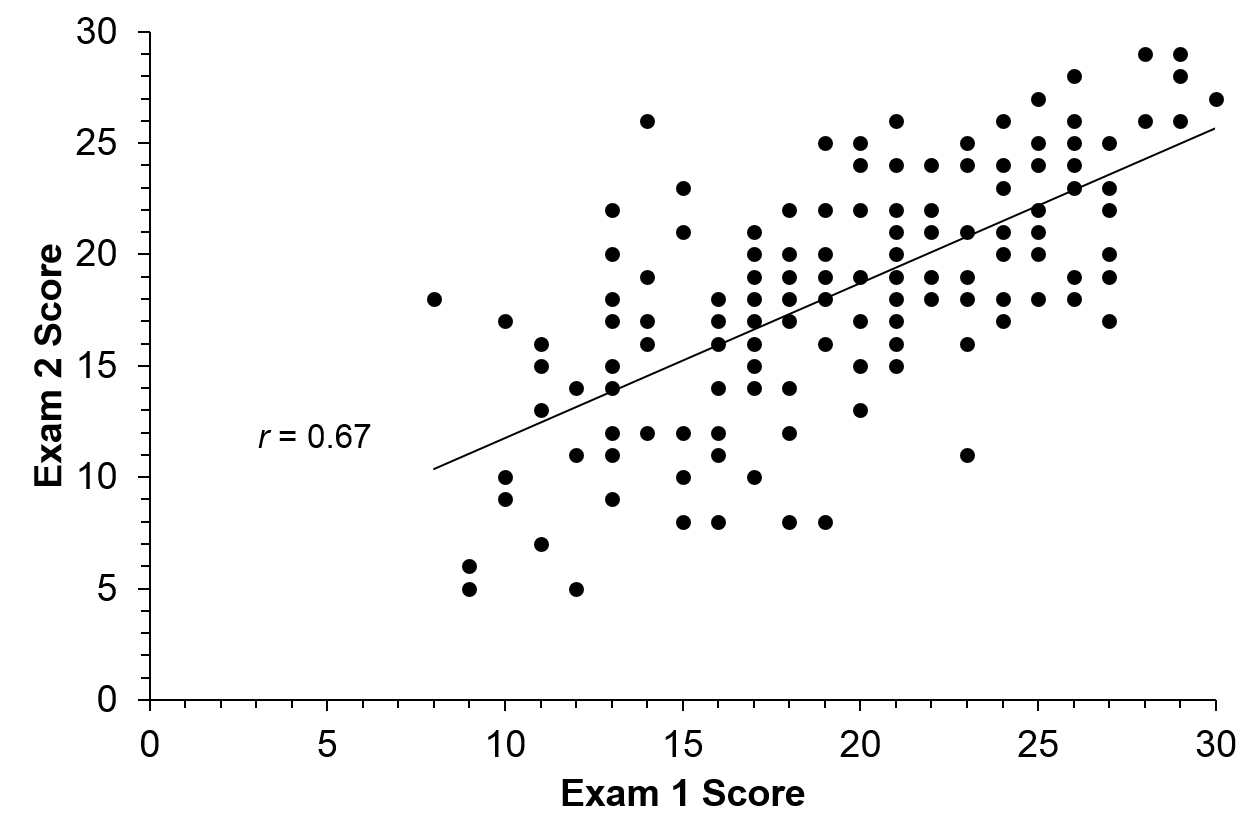
\includegraphics[width=3.5in]{restriction_range1.png}
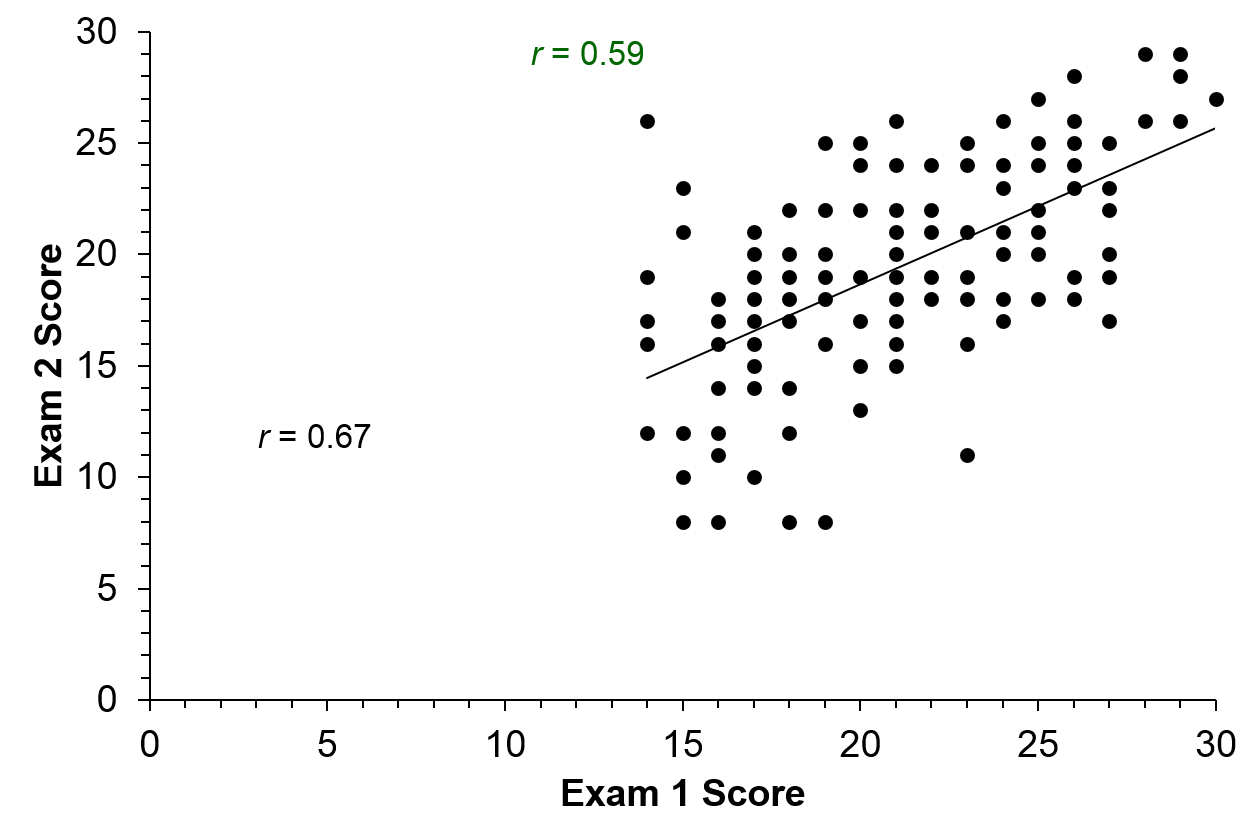
\includegraphics[width=3.5in]{restriction_range2.png}

\section{Correlations with
subpopulations}\label{correlations-with-subpopulations}

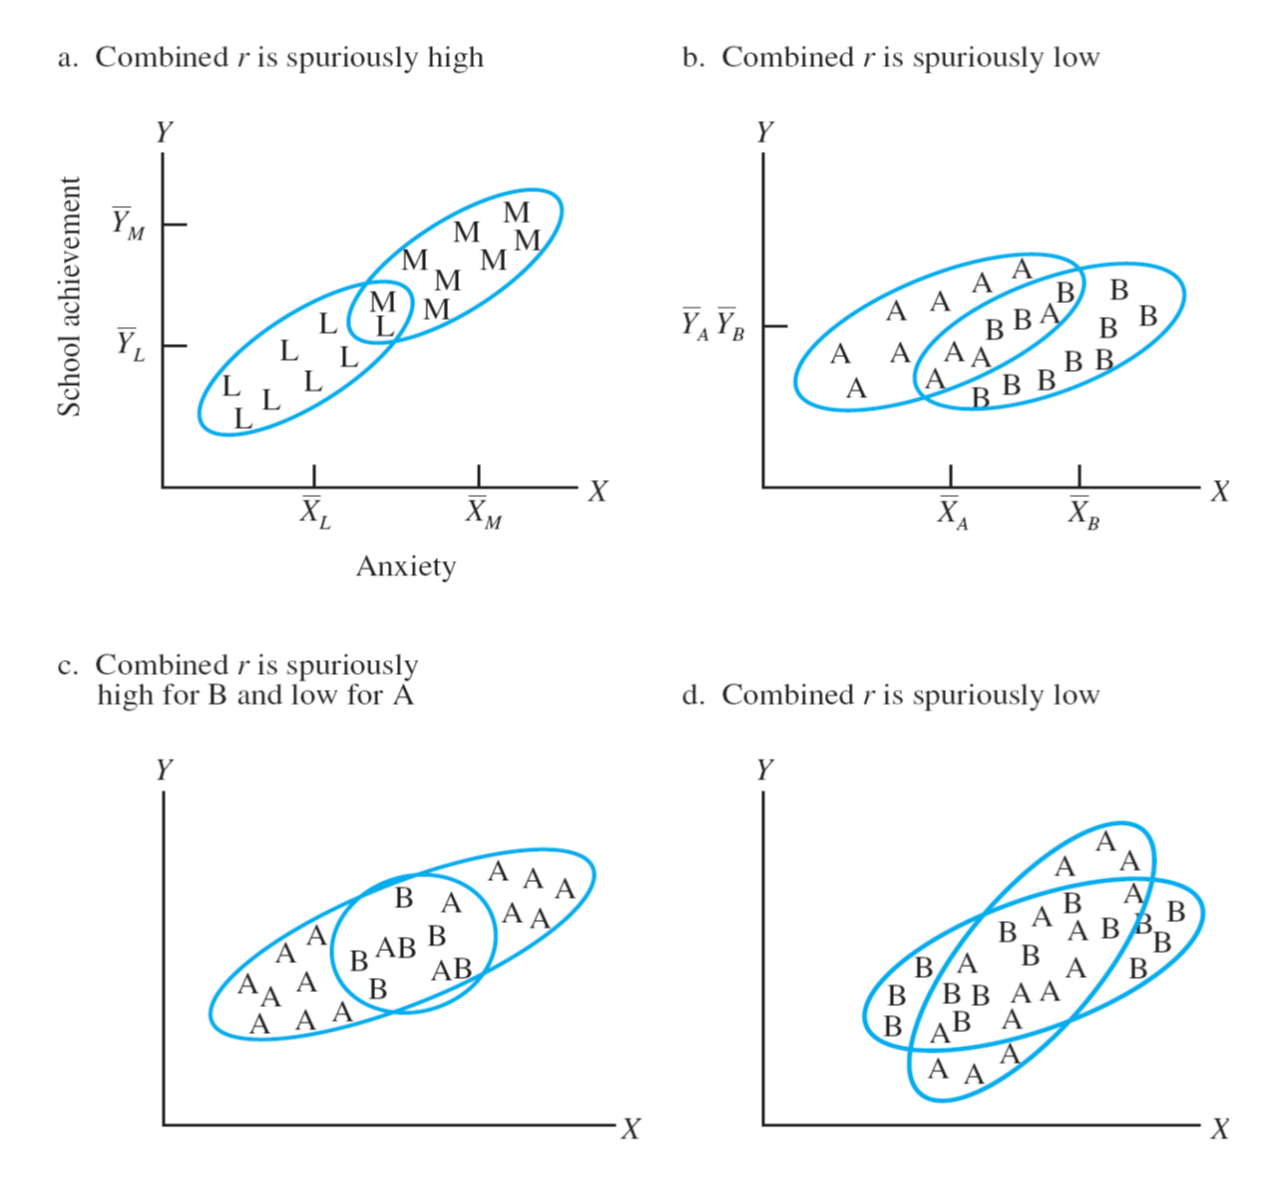
\includegraphics[width=3.5in]{corr_subpop.png} 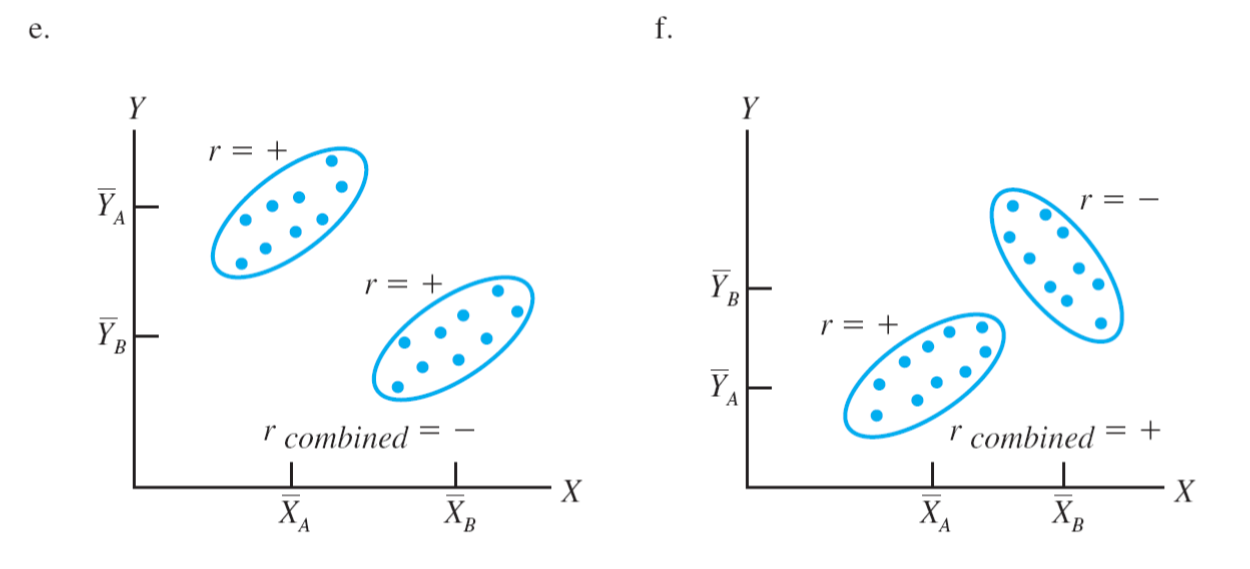
\includegraphics[width=3.5in]{corr_subpop2.png}

\section{Cautions for Correlation
Summary}\label{cautions-for-correlation-summary}

\begin{enumerate}
\def\labelenumi{\arabic{enumi}.}
\itemsep1pt\parskip0pt\parsep0pt
\item
  Careful about causation, remember correlation does not imply causation
\item
  Outliers can alter the correlation.
\item
  We discussed the correlation for \textbf{linear} relationships, not
  non-linear.
\item
  Restriction of range can decrease (attenuate) correlations.
\item
  More than one population can change the effect of the correlation.
\item
  Correlations of averages can be stronger than correlation of raw
  scores.
\end{enumerate}

\end{document}
